\documentclass[a4paper, 12pt]{article}
%%%%%%%%%%%%%%%%%%%%%%%%%%%%%%%%%%%%%%%%%%%%%%%%%%%%%%%%%%%%%%%%%%%%%%%%%%%%%%%
%                                Basic Packages                               %
%%%%%%%%%%%%%%%%%%%%%%%%%%%%%%%%%%%%%%%%%%%%%%%%%%%%%%%%%%%%%%%%%%%%%%%%%%%%%%%

% Gives us multiple colors.
\usepackage[usenames,dvipsnames,pdftex]{xcolor}
% Lets us style link colors.
\usepackage{hyperref}
% Lets us import images and graphics.
\usepackage{graphicx}
% Lets us use figures in floating environments.
\usepackage{float}
% Lets us create multiple columns.
\usepackage{multicol}
% Gives us better math syntax.
\usepackage{amsmath,amsfonts,mathtools,amsthm,amssymb}
% Lets us strikethrough text.
\usepackage{cancel}
% Lets us edit the caption of a figure.
\usepackage{caption}
% Lets us import pdf directly in our tex code.
\usepackage{pdfpages}
% Lets us do algorithm stuff.
\usepackage[ruled,vlined,linesnumbered]{algorithm2e}
% Use a smiley face for our qed symbol.
\usepackage{tikzsymbols}
% \usepackage{fullpage} %%smaller margins
\usepackage[shortlabels]{enumitem}

\setlist[enumerate]{font={\bfseries}} % global settings, for all lists

\usepackage{setspace}
\usepackage[margin=1in, headsep=12pt]{geometry}
\usepackage{wrapfig}
\usepackage{listings}
\usepackage{parskip}

\definecolor{codegreen}{rgb}{0,0.6,0}
\definecolor{codegray}{rgb}{0.5,0.5,0.5}
\definecolor{codepurple}{rgb}{0.58,0,0.82}
\definecolor{backcolour}{rgb}{0.95,0.95,0.95}

\lstdefinestyle{mystyle}{
    backgroundcolor=\color{backcolour},   
    commentstyle=\color{codegreen},
    keywordstyle=\color{magenta},
    numberstyle=\tiny\color{codegray},
    stringstyle=\color{codepurple},
    basicstyle=\ttfamily\footnotesize,
    breakatwhitespace=false,         
    breaklines=true,                 
    captionpos=b,                    
    keepspaces=true,                 
    numbers=left,                    
    numbersep=5pt,                  
    showspaces=false,                
    showstringspaces=false,
    showtabs=false,                  
    tabsize=2,
    numbers=none
}

\lstset{style=mystyle}
\def\class{article}


%%%%%%%%%%%%%%%%%%%%%%%%%%%%%%%%%%%%%%%%%%%%%%%%%%%%%%%%%%%%%%%%%%%%%%%%%%%%%%%
%                                Basic Settings                               %
%%%%%%%%%%%%%%%%%%%%%%%%%%%%%%%%%%%%%%%%%%%%%%%%%%%%%%%%%%%%%%%%%%%%%%%%%%%%%%%

%%%%%%%%%%%%%
%  Symbols  %
%%%%%%%%%%%%%

\let\implies\Rightarrow
\let\impliedby\Leftarrow
\let\iff\Leftrightarrow
\let\epsilon\varepsilon
%%%%%%%%%%%%
%  Tables  %
%%%%%%%%%%%%

\setlength{\tabcolsep}{5pt}
\renewcommand\arraystretch{1.5}

%%%%%%%%%%%%%%
%  SI Unitx  %
%%%%%%%%%%%%%%

\usepackage{siunitx}
\sisetup{locale = FR}

%%%%%%%%%%
%  TikZ  %
%%%%%%%%%%

\usepackage[framemethod=TikZ]{mdframed}
\usepackage{tikz}
\usepackage{tikz-cd}
\usepackage{tikzsymbols}

\usetikzlibrary{intersections, angles, quotes, calc, positioning}
\usetikzlibrary{arrows.meta}

\tikzset{
    force/.style={thick, {Circle[length=2pt]}-stealth, shorten <=-1pt}
}

%%%%%%%%%%%%%%%
%  PGF Plots  %
%%%%%%%%%%%%%%%

\usepackage{pgfplots}
\pgfplotsset{width=10cm, compat=newest}

%%%%%%%%%%%%%%%%%%%%%%%
%  Center Title Page  %
%%%%%%%%%%%%%%%%%%%%%%%

\usepackage{titling}
\renewcommand\maketitlehooka{\null\mbox{}\vfill}
\renewcommand\maketitlehookd{\vfill\null}

%%%%%%%%%%%%%%%%%%%%%%%%%%%%%%%%%%%%%%%%%%%%%%%%%%%%%%%
%  Create a grey background in the middle of the PDF  %
%%%%%%%%%%%%%%%%%%%%%%%%%%%%%%%%%%%%%%%%%%%%%%%%%%%%%%%

\usepackage{eso-pic}
\newcommand\definegraybackground{
    \definecolor{reallylightgray}{HTML}{FAFAFA}
    \AddToShipoutPicture{
        \ifthenelse{\isodd{\thepage}}{
            \AtPageLowerLeft{
                \put(\LenToUnit{\dimexpr\paperwidth-222pt},0){
                    \color{reallylightgray}\rule{222pt}{297mm}
                }
            }
        }
        {
            \AtPageLowerLeft{
                \color{reallylightgray}\rule{222pt}{297mm}
            }
        }
    }
}

%%%%%%%%%%%%%%%%%%%%%%%%
%  Modify Links Color  %
%%%%%%%%%%%%%%%%%%%%%%%%

\hypersetup{
    % Enable highlighting links.
    colorlinks,
    % Change the color of links to blue.
    urlcolor=blue,
    % Change the color of citations to black.
    citecolor={black},
    % Change the color of url's to blue with some black.
    linkcolor={blue!80!black}
}

%%%%%%%%%%%%%%%%%%
% Fix WrapFigure %
%%%%%%%%%%%%%%%%%%

\newcommand{\wrapfill}{\par\ifnum\value{WF@wrappedlines}>0
        \parskip=0pt
        \addtocounter{WF@wrappedlines}{-1}%
        \null\vspace{\arabic{WF@wrappedlines}\baselineskip}%
        \WFclear
    \fi}

%%%%%%%%%%%%%%%%%
% Multi Columns %
%%%%%%%%%%%%%%%%%

\let\multicolmulticols\multicols
\let\endmulticolmulticols\endmulticols

\RenewDocumentEnvironment{multicols}{mO{}}
{%
    \ifnum#1=1
        #2%
    \else % More than 1 column
        \multicolmulticols{#1}[#2]
    \fi
}
{%
    \ifnum#1=1
    \else % More than 1 column
        \endmulticolmulticols
    \fi
}

\newlength{\thickarrayrulewidth}
\setlength{\thickarrayrulewidth}{5\arrayrulewidth}


%%%%%%%%%%%%%%%%%%%%%%%%%%%%%%%%%%%%%%%%%%%%%%%%%%%%%%%%%%%%%%%%%%%%%%%%%%%%%%%
%                           School Specific Commands                          %
%%%%%%%%%%%%%%%%%%%%%%%%%%%%%%%%%%%%%%%%%%%%%%%%%%%%%%%%%%%%%%%%%%%%%%%%%%%%%%%

%%%%%%%%%%%%%%%%%%%%%%%%%%%
%  Initiate New Counters  %
%%%%%%%%%%%%%%%%%%%%%%%%%%%

\newcounter{lecturecounter}

%%%%%%%%%%%%%%%%%%%%%%%%%%
%  Helpful New Commands  %
%%%%%%%%%%%%%%%%%%%%%%%%%%

\makeatletter

\newcommand\resetcounters{
    % Reset the counters for subsection, subsubsection and the definition
    % all the custom environments.
    \setcounter{subsection}{0}
    \setcounter{subsubsection}{0}
    \setcounter{definition0}{0}
    \setcounter{paragraph}{0}
    \setcounter{theorem}{0}
    \setcounter{claim}{0}
    \setcounter{corollary}{0}
    \setcounter{proposition}{0}
    \setcounter{lemma}{0}
    \setcounter{exercise}{0}
    \setcounter{problem}{0}
    
    \setcounter{subparagraph}{0}
    % \@ifclasswith\class{nocolor}{
    %     \setcounter{definition}{0}
    % }{}
}

%%%%%%%%%%%%%%%%%%%%%
%  Lecture Command  %
%%%%%%%%%%%%%%%%%%%%%

\usepackage{xifthen}

% EXAMPLE:
% 1. \lecture{Oct 17 2022 Mon (08:46:48)}{Lecture Title}
% 2. \lecture[4]{Oct 17 2022 Mon (08:46:48)}{Lecture Title}
% 3. \lecture{Oct 17 2022 Mon (08:46:48)}{}
% 4. \lecture[4]{Oct 17 2022 Mon (08:46:48)}{}
% Parameters:
% 1. (Optional) lecture number.
% 2. Time and date of lecture.
% 3. Lecture Title.
\def\@lecture{}
\def\@lectitle{}
\def\@leccount{}
\newcommand\lecture[3]{
    \newpage

    % Check if user passed the lecture title or not.
    \def\@leccount{Lecture #1}
    \ifthenelse{\isempty{#3}}{
        \def\@lecture{Lecture #1}
        \def\@lectitle{Lecture #1}
    }{
        \def\@lecture{Lecture #1: #3}
        \def\@lectitle{#3}
    }

    \setcounter{section}{#1}
    \renewcommand\thesubsection{#1.\arabic{subsection}}
    
    \phantomsection
    \addcontentsline{toc}{section}{\@lecture}
    \resetcounters

    \begin{mdframed}
        \begin{center}
            \Large \textbf{\@leccount}
            
            \vspace*{0.2cm}
            
            \large \@lectitle
            
            
            \vspace*{0.2cm}

            \normalsize #2
        \end{center}
    \end{mdframed}

}

%%%%%%%%%%%%%%%%%%%%
%  Import Figures  %
%%%%%%%%%%%%%%%%%%%%

\usepackage{import}
\pdfminorversion=7

% EXAMPLE:
% 1. \incfig{limit-graph}
% 2. \incfig[0.4]{limit-graph}
% Parameters:
% 1. The figure name. It should be located in figures/NAME.tex_pdf.
% 2. (Optional) The width of the figure. Example: 0.5, 0.35.
\newcommand\incfig[2][1]{%
    \def\svgwidth{#1\columnwidth}
    \import{./figures/}{#2.pdf_tex}
}

\begingroup\expandafter\expandafter\expandafter\endgroup
\expandafter\ifx\csname pdfsuppresswarningpagegroup\endcsname\relax
\else
    \pdfsuppresswarningpagegroup=1\relax
\fi

%%%%%%%%%%%%%%%%%
% Fancy Headers %
%%%%%%%%%%%%%%%%%

\usepackage{fancyhdr}

% Force a new page.
\newcommand\forcenewpage{\clearpage\mbox{~}\clearpage\newpage}

% This command makes it easier to manage my headers and footers.
\newcommand\createintro{
    % Use roman page numbers (e.g. i, v, vi, x, ...)
    \pagenumbering{roman}

    % Display the page style.
    \maketitle
    % Make the title pagestyle empty, meaning no fancy headers and footers.
    \thispagestyle{empty}
    % Create a newpage.
    \newpage

    % Input the intro.tex page if it exists.
    \IfFileExists{intro.tex}{ % If the intro.tex file exists.
        % Input the intro.tex file.
        \textbf{Course}: MATH 16300: Honors Calculus III

\textbf{Section}: 43

\textbf{Professor}: Minjae Park

\textbf{At}: The University of Chicago

\textbf{Quarter}: Spring 2023

\textbf{Course materials}: Calculus by Spivak (4th Edition), Calculus On Manifolds by Spivak

\vspace{1cm}
\textbf{Disclaimer}: This document will inevitably contain some mistakes, both simple typos and serious logical and mathematical errors. Take what you read with a grain of salt as it is made by an undergraduate student going through the learning process himself. If you do find any error, I would really appreciate it if you can let me know by email at \href{mailto:conghungletran@gmail.com}{conghungletran@gmail.com}.

        % Make the pagestyle fancy for the intro.tex page.
        \pagestyle{fancy}

        % Remove the line for the header.
        \renewcommand\headrulewidth{0pt}

        % Remove all header stuff.
        \fancyhead{}

        % Add stuff for the footer in the center.
        % \fancyfoot[C]{
        %   \textit{For more notes like this, visit
        %   \href{\linktootherpages}{\shortlinkname}}. \\
        %   \vspace{0.1cm}
        %   \hrule
        %   \vspace{0.1cm}
        %   \@author, \\
        %   \term: \academicyear, \\
        %   Last Update: \@date, \\
        %   \faculty
        % }

        \newpage
    }{ % If the intro.tex file doesn't exist.
        % Force a \newpageage.
        % \forcenewpage
        \newpage
    }

    % Remove the center stuff we did above, and replace it with just the page
    % number, which is still in roman numerals.
    \fancyfoot[C]{\thepage}
    % Add the table of contents.
    \tableofcontents
    % Force a new page.
    \newpage

    % Move the page numberings back to arabic, from roman numerals.
    \pagenumbering{arabic}
    % Set the page number to 1.
    \setcounter{page}{1}

    % Add the header line back.
    \renewcommand\headrulewidth{0.4pt}
    % In the top right, add the lecture title.
    \fancyhead[R]{\footnotesize \@lecture}
    % In the top left, add the author name.
    \fancyhead[L]{\footnotesize \@author}
    % In the bottom center, add the page.
    \fancyfoot[C]{\thepage}
    % Add a nice gray background in the middle of all the upcoming pages.
    % \definegraybackground
}

\makeatother


%%%%%%%%%%%%%%%%%%%%%%%%%%%%%%%%%%%%%%%%%%%%%%%%%%%%%%%%%%%%%%%%%%%%%%%%%%%%%%%
%                               Custom Commands                               %
%%%%%%%%%%%%%%%%%%%%%%%%%%%%%%%%%%%%%%%%%%%%%%%%%%%%%%%%%%%%%%%%%%%%%%%%%%%%%%%

%%%%%%%%%%%%
%  Circle  %
%%%%%%%%%%%%

\newcommand*\circled[1]{\tikz[baseline= (char.base)]{
        \node[shape=circle,draw,inner sep=1pt] (char) {#1};}
}

%%%%%%%%%%%%%%%%%%%
%  Todo Commands  %
%%%%%%%%%%%%%%%%%%%

% \usepackage{xargs}
% \usepackage[colorinlistoftodos]{todonotes}

% \makeatletter

% \@ifclasswith\class{working}{
%     \newcommandx\unsure[2][1=]{\todo[linecolor=red,backgroundcolor=red!25,bordercolor=red,#1]{#2}}
%     \newcommandx\change[2][1=]{\todo[linecolor=blue,backgroundcolor=blue!25,bordercolor=blue,#1]{#2}}
%     \newcommandx\info[2][1=]{\todo[linecolor=OliveGreen,backgroundcolor=OliveGreen!25,bordercolor=OliveGreen,#1]{#2}}
%     \newcommandx\improvement[2][1=]{\todo[linecolor=Plum,backgroundcolor=Plum!25,bordercolor=Plum,#1]{#2}}

%     \newcommand\listnotes{
%         \newpage
%         \listoftodos[Notes]
%     }
% }{
%     \newcommandx\unsure[2][1=]{}
%     \newcommandx\change[2][1=]{}
%     \newcommandx\info[2][1=]{}
%     \newcommandx\improvement[2][1=]{}

%     \newcommand\listnotes{}
% }

% \makeatother

%%%%%%%%%%%%%
%  Correct  %
%%%%%%%%%%%%%

% EXAMPLE:
% 1. \correct{INCORRECT}{CORRECT}
% Parameters:
% 1. The incorrect statement.
% 2. The correct statement.
\definecolor{correct}{HTML}{009900}
\newcommand\correct[2]{{\color{red}{#1 }}\ensuremath{\to}{\color{correct}{ #2}}}


%%%%%%%%%%%%%%%%%%%%%%%%%%%%%%%%%%%%%%%%%%%%%%%%%%%%%%%%%%%%%%%%%%%%%%%%%%%%%%%
%                                 Environments                                %
%%%%%%%%%%%%%%%%%%%%%%%%%%%%%%%%%%%%%%%%%%%%%%%%%%%%%%%%%%%%%%%%%%%%%%%%%%%%%%%

\usepackage{varwidth}
\usepackage{thmtools}
\usepackage[most,many,breakable]{tcolorbox}

\tcbuselibrary{theorems,skins,hooks}
\usetikzlibrary{arrows,calc,shadows.blur}

%%%%%%%%%%%%%%%%%%%
%  Define Colors  %
%%%%%%%%%%%%%%%%%%%

% color prototype
% \definecolor{color}{RGB}{45, 111, 177}

% ESSENTIALS: 
\definecolor{myred}{HTML}{c74540}
\definecolor{myblue}{HTML}{072b85}
\definecolor{mygreen}{HTML}{388c46}
\definecolor{myblack}{HTML}{000000}

\colorlet{definition_color}{myred}

\colorlet{theorem_color}{myblue}
\colorlet{lemma_color}{myblue}
\colorlet{prop_color}{myblue}
\colorlet{corollary_color}{myblue}
\colorlet{claim_color}{myblue}

\colorlet{proof_color}{myblack}
\colorlet{example_color}{myblack}
\colorlet{exercise_color}{myblack}

% MISCS: 
%%%%%%%%%%%%%%%%%%%%%%%%%%%%%%%%%%%%%%%%%%%%%%%%%%%%%%%%%
%  Create Environments Styles Based on Given Parameter  %
%%%%%%%%%%%%%%%%%%%%%%%%%%%%%%%%%%%%%%%%%%%%%%%%%%%%%%%%%

% \mdfsetup{skipabove=1em,skipbelow=0em}

%%%%%%%%%%%%%%%%%%%%%%
%  Helpful Commands  %
%%%%%%%%%%%%%%%%%%%%%%

% EXAMPLE:
% 1. \createnewtheoremstyle{thmdefinitionbox}{}{}
% 2. \createnewtheoremstyle{thmtheorembox}{}{}
% 3. \createnewtheoremstyle{thmproofbox}{qed=\qedsymbol}{
%       rightline=false, topline=false, bottomline=false
%    }
% Parameters:
% 1. Theorem name.
% 2. Any extra parameters to pass directly to declaretheoremstyle.
% 3. Any extra parameters to pass directly to mdframed.
\newcommand\createnewtheoremstyle[3]{
    \declaretheoremstyle[
        headfont=\bfseries\sffamily, bodyfont=\normalfont, #2,
        mdframed={
                #3,
            },
    ]{#1}
}

% EXAMPLE:
% 1. \createnewcoloredtheoremstyle{thmdefinitionbox}{definition}{}{}
% 2. \createnewcoloredtheoremstyle{thmexamplebox}{example}{}{
%       rightline=true, leftline=true, topline=true, bottomline=true
%     }
% 3. \createnewcoloredtheoremstyle{thmproofbox}{proof}{qed=\qedsymbol}{backgroundcolor=white}
% Parameters:
% 1. Theorem name.
% 2. Color of theorem.
% 3. Any extra parameters to pass directly to declaretheoremstyle.
% 4. Any extra parameters to pass directly to mdframed.

% change backgroundcolor to #2!5 if user wants a colored backdrop to theorem environments. It's a cool color theme, but there's too much going on in the page.
\newcommand\createnewcoloredtheoremstyle[4]{
    \declaretheoremstyle[
        headfont=\bfseries\sffamily\color{#2},
        bodyfont=\normalfont,
        headpunct=,
        headformat = \NAME~\NUMBER\NOTE \hfill\smallskip\linebreak,
        #3,
        mdframed={
                outerlinewidth=0.75pt,
                rightline=false,
                leftline=false,
                topline=false,
                bottomline=false,
                backgroundcolor=white,
                skipabove = 5pt,
                skipbelow = 0pt,
                linecolor=#2,
                innertopmargin = 0pt,
                innerbottommargin = 0pt,
                innerrightmargin = 4pt,
                innerleftmargin= 6pt,
                leftmargin = -6pt,
                #4,
            },
    ]{#1}
}



%%%%%%%%%%%%%%%%%%%%%%%%%%%%%%%%%%%
%  Create the Environment Styles  %
%%%%%%%%%%%%%%%%%%%%%%%%%%%%%%%%%%%

\makeatletter
\@ifclasswith\class{nocolor}{
    % Environments without color.

    % ESSENTIALS:
    \createnewtheoremstyle{thmdefinitionbox}{}{}
    \createnewtheoremstyle{thmtheorembox}{}{}
    \createnewtheoremstyle{thmproofbox}{qed=\qedsymbol}{}
    \createnewtheoremstyle{thmcorollarybox}{}{}
    \createnewtheoremstyle{thmlemmabox}{}{}
    \createnewtheoremstyle{thmclaimbox}{}{}
    \createnewtheoremstyle{thmexamplebox}{}{}

    % MISCS: 
    \createnewtheoremstyle{thmpropbox}{}{}
    \createnewtheoremstyle{thmexercisebox}{}{}
    \createnewtheoremstyle{thmexplanationbox}{}{}
    \createnewtheoremstyle{thmremarkbox}{}{}
    
    % STYLIZED MORE BELOW
    \createnewtheoremstyle{thmquestionbox}{}{}
    \createnewtheoremstyle{thmsolutionbox}{qed=\qedsymbol}{}
}{
    % Environments with color.

    % ESSENTIALS: definition, theorem, proof, corollary, lemma, claim, example
    \createnewcoloredtheoremstyle{thmdefinitionbox}{definition_color}{}{leftline=false}
    \createnewcoloredtheoremstyle{thmtheorembox}{theorem_color}{}{leftline=false}
    \createnewcoloredtheoremstyle{thmproofbox}{proof_color}{qed=\qedsymbol}{}
    \createnewcoloredtheoremstyle{thmcorollarybox}{corollary_color}{}{leftline=false}
    \createnewcoloredtheoremstyle{thmlemmabox}{lemma_color}{}{leftline=false}
    \createnewcoloredtheoremstyle{thmpropbox}{prop_color}{}{leftline=false}
    \createnewcoloredtheoremstyle{thmclaimbox}{claim_color}{}{leftline=false}
    \createnewcoloredtheoremstyle{thmexamplebox}{example_color}{}{}
    \createnewcoloredtheoremstyle{thmexplanationbox}{example_color}{qed=\qedsymbol}{}
    \createnewcoloredtheoremstyle{thmremarkbox}{theorem_color}{}{}

    \createnewcoloredtheoremstyle{thmmiscbox}{black}{}{}

    \createnewcoloredtheoremstyle{thmexercisebox}{exercise_color}{}{}
    \createnewcoloredtheoremstyle{thmproblembox}{theorem_color}{}{leftline=false}
    \createnewcoloredtheoremstyle{thmsolutionbox}{mygreen}{qed=\qedsymbol}{}
}
\makeatother

%%%%%%%%%%%%%%%%%%%%%%%%%%%%%
%  Create the Environments  %
%%%%%%%%%%%%%%%%%%%%%%%%%%%%%
\declaretheorem[numberwithin=section, style=thmdefinitionbox,     name=Definition]{definition}
\declaretheorem[numberwithin=section, style=thmtheorembox,     name=Theorem]{theorem}
\declaretheorem[numbered=no,          style=thmexamplebox,     name=Example]{example}
\declaretheorem[numberwithin=section, style=thmtheorembox,       name=Claim]{claim}
\declaretheorem[numberwithin=section, style=thmcorollarybox,   name=Corollary]{corollary}
\declaretheorem[numberwithin=section, style=thmpropbox,        name=Proposition]{proposition}
\declaretheorem[numberwithin=section, style=thmlemmabox,       name=Lemma]{lemma}
\declaretheorem[numberwithin=section, style=thmexercisebox,    name=Exercise]{exercise}
\declaretheorem[numbered=no,          style=thmproofbox,       name=Proof]{proof0}
\declaretheorem[numbered=no,          style=thmexplanationbox, name=Explanation]{explanation}
\declaretheorem[numbered=no,          style=thmsolutionbox,    name=Solution]{solution}
\declaretheorem[numberwithin=section,          style=thmproblembox,     name=Problem]{problem}
\declaretheorem[numbered=no,          style=thmmiscbox,    name=Intuition]{intuition}
\declaretheorem[numbered=no,          style=thmmiscbox,    name=Goal]{goal}
\declaretheorem[numbered=no,          style=thmmiscbox,    name=Recall]{recall}
\declaretheorem[numbered=no,          style=thmmiscbox,    name=Motivation]{motivation}
\declaretheorem[numbered=no,          style=thmmiscbox,    name=Remark]{remark}
\declaretheorem[numbered=no,          style=thmmiscbox,    name=Observe]{observe}
\declaretheorem[numbered=no,          style=thmmiscbox,    name=Question]{question}


%%%%%%%%%%%%%%%%%%%%%%%%%%%%
%  Edit Proof Environment  %
%%%%%%%%%%%%%%%%%%%%%%%%%%%%

\renewenvironment{proof}[2][\proofname]{
    % \vspace{-12pt}
    \begin{proof0} [#2]
        }{\end{proof0}}

\theoremstyle{definition}

\newtheorem*{notation}{Notation}
\newtheorem*{previouslyseen}{As previously seen}
\newtheorem*{property}{Property}
% \newtheorem*{intuition}{Intuition}
% \newtheorem*{goal}{Goal}
% \newtheorem*{recall}{Recall}
% \newtheorem*{motivation}{Motivation}
% \newtheorem*{remark}{Remark}
% \newtheorem*{observe}{Observe}

\author{Hung C. Le Tran}


%%%% MATH SHORTHANDS %%%%
%% blackboard bold math capitals
\DeclareMathOperator*{\esssup}{ess\,sup}
\DeclareMathOperator*{\Hom}{Hom}
\newcommand{\bbf}{\mathbb{F}}
\newcommand{\bbn}{\mathbb{N}}
\newcommand{\bbq}{\mathbb{Q}}
\newcommand{\bbr}{\mathbb{R}}
\newcommand{\bbz}{\mathbb{Z}}
\newcommand{\bbc}{\mathbb{C}}
\newcommand{\bbk}{\mathbb{K}}
\newcommand{\bbm}{\mathbb{M}}
\newcommand{\bbp}{\mathbb{P}}
\newcommand{\bbe}{\mathbb{E}}

\newcommand{\bfw}{\mathbf{w}}
\newcommand{\bfx}{\mathbf{x}}
\newcommand{\bfX}{\mathbf{X}}
\newcommand{\bfy}{\mathbf{y}}
\newcommand{\bfyhat}{\mathbf{\hat{y}}}

\newcommand{\calb}{\mathcal{B}}
\newcommand{\calf}{\mathcal{F}}
\newcommand{\calt}{\mathcal{T}}
\newcommand{\call}{\mathcal{L}}
\renewcommand{\phi}{\varphi}

% Universal Math Shortcuts
\newcommand{\st}{\hspace*{2pt}\text{s.t.}\hspace*{2pt}}
\newcommand{\pffwd}{\hspace*{2pt}\fbox{\(\Rightarrow\)}\hspace*{10pt}}
\newcommand{\pfbwd}{\hspace*{2pt}\fbox{\(\Leftarrow\)}\hspace*{10pt}}
\newcommand{\contra}{\ensuremath{\Rightarrow\Leftarrow}}
\newcommand{\cvgn}{\xrightarrow{n \to \infty}}
\newcommand{\cvgj}{\xrightarrow{j \to \infty}}

\newcommand{\im}{\mathrm{im}}
\newcommand{\innerproduct}[2]{\langle #1, #2 \rangle}
\newcommand*{\conj}[1]{\overline{#1}}

% https://tex.stackexchange.com/questions/438612/space-between-exists-and-forall
% https://tex.stackexchange.com/questions/22798/nice-looking-empty-set
\let\oldforall\forall
\renewcommand{\forall}{\;\oldforall\; }
\let\oldexist\exists
\renewcommand{\exists}{\;\oldexist\; }
\newcommand\existu{\;\oldexist!\: }
\let\oldemptyset\emptyset
\let\emptyset\varnothing


\renewcommand{\_}[1]{\underline{#1}}
\DeclarePairedDelimiter{\abs}{\lvert}{\rvert}
\DeclarePairedDelimiter{\norm}{\lVert}{\rVert}
\DeclarePairedDelimiter\ceil{\lceil}{\rceil}
\DeclarePairedDelimiter\floor{\lfloor}{\rfloor}
\setlength\parindent{0pt}
\setlength{\headheight}{12.0pt}
\addtolength{\topmargin}{-12.0pt}


% Default skipping, change if you want more spacing
% \thinmuskip=3mu
% \medmuskip=4mu plus 2mu minus 4mu
% \thickmuskip=5mu plus 5mu

% \DeclareMathOperator{\ext}{ext}
% \DeclareMathOperator{\bridge}{bridge}
\title{MATH 20700: Honors Analysis in Rn I \\ \large Problem Set 7}
\date{12 Nov 2023}
\author{Hung Le Tran}
\begin{document}
\maketitle
\setcounter{section}{7}
\textbf{Textbook: Pugh's Real Mathematical Analysis}

\textit{Collaborators: Lucio, Hung Pham, Duc}

\begin{problem} [5.32 \redtext{done}]
Let $G$ denote the set of invertible $n \times n$ matrices.
\begin{enumerate} [(a)]
    \item Prove that $G$ is an open subset of $\calm(n \times n)$
    \item Prove that $G$ is a group.
    \item Prove that the inversion operator $Inv: A \mapsto A^{-1}$ is a homeomorphism of $G$ onto $G$.
    \item Prove that $Inv$ is a diffeomorphism and show that its derivative at $A$ is the linear transformation $\calm \to \calm$, \[
              X \mapsto -A^{-1} \circ X \circ A^{-1}.
          \]
    \item Relate this formula to the ordinary derivative of $1/x$ at $x = a$.
\end{enumerate}
\end{problem}
\begin{solution}
    \textbf{(a)} Consider the determinant function: \[
        \det: \calm(n \times n) \to \bbr, M \mapsto \det(M)
    \]

    Using the Frobenius norm (essentially Euclidean norm on $\bbr^{n^2}$) on $\calm(n \times n)$, $\det$ is continuous because it is a polynomial in the entries of $M$:
    \[
        \det M = \sum_{\pi} sgn(\pi) M_{1\pi(1)} M_{2\pi(2)}\ldots M_{n\pi(n)}
    \]
    We also know that $\bbr \backslash \{0\}$ is open in $\bbr$, since its complement $\{0\}$ is closed. Therefore $\det^{Pre}(\bbr\backslash \{0\})$ is open in $\calm(n \times n)$.

    Matrices are invertible iff their determinant is non-zero, so the group of invertible matrices is exactly $\det^{Pre}(\bbr\backslash \{0\})$, which is open as required. \qed

    \textbf{(b)} WTS $G$ is a group, with matrix multiplication as the group operation.

    \textbf{1.} There exists an identity element, namely $I = I_{n \times n}$. $I$ is clearly invertible. Then, for all $M \in G$, \[
        IM = MI = M
    \]

    \textbf{2.} For all $M \in G$, there exists an inverse, namely, $M^{-1}$. $M^{-1} \in G$ because it is invertible, its inverse is $M$. And (essentially restating this fact, but in the context of the group)\[
        M M^{-1} = M^{-1} M = I \:\text{(Group Identity)}\:
    \]

    \textbf{3.} $G$ is closed under the group operation. Let $A, B \in G$ then $AB \in G$ too, since $\det (AB) = \det A \det B \neq 0$.

    \textbf{4.} The group operation is associative, because matrix multiplication is associative.

    Therefore $G$ is a group. \qed

    % \textbf{(c)} WTS $Inv: G \to G, A \mapsto A^{-1}$ is a homeomorphism.


    % $A^{-1} = \frac{A'}{\det(A)}$, where $A'$ is the adjugate matrix of $A$. The entries of $A'$ are determinants of some collection of entries of $A$ divided by $\det A$, which is essentially a rational function of the entries of $A$. It follows that $A \mapsto A^{-1}$ is continuous.

    % It is clearly a bijection, since there exists an inverse function, which is itself: \[
    % Inv \circ Inv = id
    % \]
    % Its inverse (itself) is continuous. It is therefore a homeomorphism. \qed

    \textbf{(c)} WTS $Inv: G \to G, A \mapsto A^{-1}$ is a homeomorphism.

    \textbf{1.} It is clearly a bijection, since there exists an inverse function, which is itself: \[
        Inv \circ Inv = id
    \]

    \textbf{2.} WTS that it is continuous. First note that for all $A \in G$, since $A \neq 0$, $\norm{A}, \norm{A^{-1}} > 0$. Fix $\epsilon > 0$. Then, using the operator norm,
    \begin{align*}
        \norm{Inv(A) - Inv(B)} & = \norm{A^{-1} - B^{-1}}                                                     \\
                               & = \norm{A^{-1}(B - A)B^{-1}}                                                 \\
                               & \leq \norm{B - A} \norm{A^{-1}B^{-1}}                                        \\
                               & \leq \norm{B-A} \norm{A^{-1}} (\norm{A^{-1}} + \norm{A^{-1} - B^{-1}})       \\
                               & = \norm{B-A} \norm{A^{-1}}^2 + \norm{B-A}\norm{A^{-1}}\norm{A^{-1} - B^{-1}}
    \end{align*}
    Grouping together terms with $\norm{A^{-1} - B^{-1}}$:
    \begin{equation*}
        \norm{A^{-1} - B^{-1}} (1 - \norm{B-A}\norm{A^{-1}})\leq \norm{B-A} \norm{A^{-1}}^2
    \end{equation*}

    Pick $\delta = \min \left\{ \frac{1}{2\norm{A^{-1}}}, \frac{\epsilon}{\norm{A^{-1}}^2} \right\}$, then if $\norm{B-A} < \delta$ then $1 - \norm{B-A}\norm{A^{-1}} > 0$, so we can divide that in both sides, then \[
        \norm{A^{-1} - B^{-1}} \leq \frac{\norm{B-A} \norm{A^{-1}}^2}{1 - \norm{B-A} \norm{A^{-1}}} \leq \frac{\norm{B-A} \norm{A^{-1}}^2}{1} \leq \delta \norm{A^{-1}}^2 \leq \epsilon
    \]

    $Inv$ is therefore continuous. \qed

    \textbf{(d)} WTS $Inv$ is a diffeomorphism.

    We write out the remainder term, if we use $X \mapsto -A^{-1}XA^{-1}$ as the linear approximation:
    \begin{align*}
        \norm{R(H)}                           & = \norm{(A+H)^{-1} - (A^{-1} - A^{-1}HA^{-1}) }       \\
                                              & = \norm{(A+H)^{-1} - A^{-1} + A^{-1}HA^{-1}}          \\
                                              & = \norm{(A+H)^{-1}(A - (A+H)) A^{-1} + A^{-1}HA^{-1}} \\
                                              & = \norm{-(A+H)^{-1}HA^{-1} + A^{-1}HA^{-1}}           \\
                                              & = \norm{(A^{-1} - (A+H)^{-1})HA^{-1}}                 \\
                                              & \leq \norm{A^{-1} - (A+H)^{-1}}\norm{H} \norm{A^{-1}} \\
        \implies \frac{\norm{R(H)}}{\norm{H}} & \leq \norm{(A+H)^{-1} - A^{-1}}\norm{A^{-1}}
    \end{align*}
    Since $Inv$ is continuous, $\lim_{H \to 0}\norm{(A+H)^{-1} - A^{-1}} = 0$, therefore $R(H)$ is indeed sublinear.

    It remains for us to show that $DInv: A \mapsto (X \mapsto -A^{-1}XA^{-1})$ is continuous.

    Fix $\epsilon > 0$. Choose $\epsilon_1$ such that $\epsilon_1 (2\norm{A^{-1}} + \epsilon_1) < \epsilon$. Then since $Inv$ is continuous, there exists $\delta$ such that $\norm{B-A} < \delta \implies \norm{Inv(B) - Inv(A)|}< \epsilon_1$. Then, since \[
        \norm{DInv_A - DInv_B} = \sup \frac{\norm{(DInv_A - DInv_B)(X)}}{\norm{X}}
    \]
    we can estimate:
    \begin{align*}
        \norm{(DInv_A - DInv_B)(X)} & = \norm{-A^{-1}XA^{-1} + B^{-1}XB^{-1}}                                                        \\
                                    & = \norm{-A^{-1}XA^{-1} + B^{-1}XA^{-1} - B^{-1}XA^{-1} + B^{-1}XB^{-1}}                        \\
                                    & = \norm{(B^{-1} - A^{-1})XA^{-1} + B^{-1}X(B^{-1} - A^{-1})}                                   \\
                                    & \leq \norm{B^{-1} - A^{-1}}\norm{X}\norm{A^{-1}} + \norm{B^{-1}}\norm{X}\norm{B^{-1} - A^{-1}} \\
                                    & \leq \norm{B^{-1} - A^{-1}}\norm{X} (\norm{A^{-1}} + \norm{A^{-1}} + \norm{B^{-1} - A^{-1}})   \\
                                    & \leq \epsilon_1 \norm{X} (2\norm{A^{-1}} + \epsilon_1)
    \end{align*}
    which implies \[
        \norm{DInv_A - DInv_B} \leq \epsilon_1 (2\norm{A^{-1}} + \epsilon_1) < \epsilon
    \]

    It follows that $DInv$ is continuous, making $Inv$ $C^1$. It is its own inverse, so it is a diffeomorphism. \qed

    \textbf{(e)}
    \[
        \frac{d}{dx}\left(\frac{1}{x}\right)\bigg|_a = -a^{-2}
    \]
    So the transformation is \[
        x \mapsto -a^{-2}x = -a^{-1} x a^{-1}
    \]
    as part (d) suggests.
\end{solution}

\begin{problem} [5.33 \redtext{done}]
Observe that $Y = Inv (X)$ solves the implicit function problem \[
    F(X, Y) - I = 0
\]
where $F(X, Y) = X \circ Y$. Assume it is known that $Inv$ is smooth and use the Chain Rule to derive from this equation the formula for the derivative of $Inv$.
\end{problem}
\begin{solution}
    It is already assumed that $Inv$ is smooth.

    Apply Leibnitz Rule:
    \begin{align*}
        0          & = F(X, Y) - I                               \\
                   & = (F (Id, Inv))(X) - I                \\
        \implies 0 & = D(F(Id, Inv))_{A}(X)                      \\
                   & = F(DId_A(X), Inv(A)) + F(Id(A), DInv_A(X))
    \end{align*}
    $Id$ is linear, so $DId_A(X) = Id(X) = X$. Therefore \[
        X A^{-1} + A (DInv_A(X)) = 0 \implies A (DInv_A(X)) = - X A^{-1} \implies DInv_A(X) = -A^{-1} X A^{-1}
    \]
\end{solution}

\begin{problem} [III \redtext{done}]
Let $f\colon B^m(0,1)\to \bbr^m$ be a $C^1$ map with the property that for every $p\in \bbr^m$,
\[\det(J_p f)\neq 0.
\]
(where $J_p f$ is the Jacobian matrix of $f$ at $p$).
\begin{enumerate}
    \item[(a)] Prove that if $\det(J_0f) > 0$, then  $\det(J_p f)> 0$, for all $p\in  B^m(0,1)$.
    \item[(b)] Prove that there exist $p,q\in  B^m(0,1)$ such that $|f(p)|\neq |f(q)|$.
\end{enumerate}
\end{problem}
\begin{solution}
    \textbf{(a)} Since $f$ is $C^1$, $Df: B^m(0, 1) \to \call(B^m(0, 1), \bbr^m); x \mapsto Df_x$ is continuous.

    There also exists a natural isomorphism that maps a linear map to its matrix representation in the standard basis, \[
        T: \call(B^m(0, 1), \bbr^m) \to M(m \times m); g \mapsto T_g
    \]
    It is an isomorphism between 2 finite dimensional vector spaces, so it is a homeomorphism.

    Lastly, \[
        \det: M(m \times m) \to \bbr; A \mapsto \det(A)
    \]
    is also continuous, since $\det (A)$ is simply a polynomial in the entries of $A$.

    It follows that the map \[
        h = \det \circ T \circ Df: B^m(0, 1) \to \bbr; x \mapsto \det(Jf_x)
    \]
    is continuous.

    With $h$ defined as such, the given conditions are translated to: $h(p) \neq 0 \forall p \in \bbr^m, h(0) > 0$.

    Then for all $p \in B^m(0, 1)$, inspect the segment $[0, p] \subset B^m(0, 1)$, which is connected.

    Suppose for sake of contradiction that $h(p) < 0$. It is given that $h(0) > 0$, so using the Generalized Intermediate Value Theorem, there exists $q \in [0, p] \subset B^m(0, 1)$ such that $h(q) = 0 \implies \det(Jf_q) = 0$, \contra

    Therefore $h(p) > 0$, i.e., $ \det(Jf_p) > 0 \forall p \in B^m(0, 1)$. \qed

    \textbf{(b)} Suppose there doesn't exist such $p, q \in B^m(0, 1)$. This implies there exists $C \in \bbr_{\geq 0}$ such that \[
        |f(x)| = C \forall x \in B^m(0, 1)
    \]

    If $C = 0 \implies f(x) = 0 \forall x \in B^m(0, 1) \implies Jf_0 = 0 \contra$

    Therefore $C > 0, f(x) \neq 0$ in $B^m(0, 1)$.

    Consider the fixed $v \in \bbr^m, v = Df_0^{-1}(f(0))$, i.e., $Df_0(v) = f(0)$. Then for $t < 0$ such that $|t| < \min\{1/|v|, 1/2\}$, we then have that $tv \in B^m (0, 1)$.

    The estimation for $tv$ would then be:
    \begin{align*}
        f(tv)                   & = f(0) + Df_0(tv) + R(tv)                     \\
                                & = f(0) + tf(0) + R(tv)                        \\
                                & = (1+t) f(0) + R(tv)                          \\
        \implies |f(tv)|        & \leq (1+t)|f(0)| + |R(tv)|                    \\
        |f(0)|                  & \leq (1+t)|f(0)| + |R(tv)|                  \\
        \implies -t|f(0)|       & \leq |R(tv)|                                  \\
        \implies 0 < C = |f(0)| & \leq \frac{|R(tv)|}{-t} = \frac{|R(tv)|}{|t|}
    \end{align*}
    so $R$ is not sublinear as $|t| \to 0$.

    It follows that there must exist $p, q \in B^m(0, 1)$ such that $|f(p)| \neq |f(q)|$.
\end{solution}


\begin{problem} [IV \redtext{done}]
Let $U\subset \bbr^n$, and let $f\colon U\to \bbr$ be a  $C^1$ function. Let  $F\colon U\to \bbr^n$ be the gradient vector field of $f$:
\[F(p) = \operatorname{grad}_p(f),
\]
for $p\in U$.
\begin{enumerate}
    \item[(a)]  Suppose that $f$ is twice differentiable at some $p\in U$, and  let  $H_p(f)\in {\mathcal M}_{n\times n}$ be the Jacobian matrix for $F$ at $p$, with respect to the standard basis $e_1,\ldots, e_n$ of $\bbr^n$ (i.e., $H_p(f)$ is $DF_p$, expressed with respect to the standard basis of $\bbr^n$).   Show that
        \[(H_p(f))_{i,j} = \frac{\partial^2 f}{\partial x_i \partial x_j}(p).
        \]
        The matrix $H_p(f)$ is called the {\em Hessian} of $f$ at $p$.
    \item[(b)] Show that, with respect to the standard basis $e_1, \ldots, e_n$ of $\bbr^n$, we have
        \[D^2f_p(v,w) = v^t H_p(f)  w,\]
        for all $v,w\in\bbr^n$, and that $H_p(f)$ is a symmetric matrix.
    \item[(c)] Show that
        \[
            f(p+h) = f(p) + \langle \operatorname{grad}_p(f), h \rangle  + \frac{1}{2} h^t H_p( f) h + R^{(2)}(p,h),
        \]
        where
        \[\lim_{h\to 0} \frac{R^{(2)}(p,h)}{|h|^2} = 0.
        \]
    \item[(d)] We say that $p$ is a {\em critical point of $f$} if $f$ is differentiable at $p$ and $F(p)=0$.  If $p$ is a  critical point of $f$, then
        \begin{equation}\label{e=criticalHess}
            f(p+h) = f(p) + \frac{1}{2}h^t H_p (f)  h + R^{(2)}(p,h),
        \end{equation}
        for all $h$ close to $0\in \bbr^n$.
        We say that a critical point $p$ is {\em nondegenerate} if $f$ is twice differentiable at $p$, and  $H_p(f)$ is invertible (or equivalently, $\det(H_p(f))\neq 0$).

        Find all critical points of the function \[f(x,y) =  2x^3 + xy^2 + 5x^2 + y^2,\] and compute the Hessian at these points.  Determine whether they are nondegenerate.

    \item[(e)] Let $A\in {\mathcal M}_{n\times n}$.  A nonzero vector $v\in \bbr^n$ is called an {\em real eigenvector} of $A$ if there exists a real number $\lambda\in\bbr$ such that $Av = \lambda v$.  The number $\lambda$ is called a {\em real eigenvalue of $A$}. 	Prove that if $A$ is a symmetric matrix (meaning $A^t = A$) and  $v_1, v_2\in\bbr\setminus \{0\}$ are real eigenvectors of $A$ with eigenvalues $\lambda_1, \lambda_2\in \bbr$, respectively, then
        \[\lambda_1\neq \lambda_2 \implies \langle v_1,v_2\rangle = 0;\]
        that is, eigenvectors for different eigenvalues are orthogonal.  (Hint: use the fact that $ \langle v_1,v_2\rangle = v_1^t v_2$).
    \item[(f)] For the function $f$ in part (d), characterize each nondegnerate critical point $p$:

        \begin{itemize}
            \item[(i)] Is $p$ a local maximum?  If so, in what directions (moving away from $p$) does the function decrease most sharply (on an infinitesimal level)?
            \item[(ii)] Is $p$ a local minimum?  If so, in what directions (moving away from $p$) does the function increase most sharply (on an infinitesimal level)?
            \item[(iii)] If $p$ is neither a local max nor a local min, determine the directions of maximal increase/decrease of $f$ at $p$.
        \end{itemize}

        Note that  you cannot use the gradient to answer these questions,  since the gradient is $0$ at these points. Instead, you will need to use equation \eqref{e=criticalHess} above, plus some linear algebra. If you have not seen eigenvectors and diagonalization before, talk to your linear algebra buddy!
\end{enumerate}
\end{problem}
\begin{solution}
    \textbf{(a)} Recall that \[
        F(p) = grad_p(f) = Jf_p^T = \begin{pmatrix}
            \partial f/\partial x_1 (p) \\
            \partial f/\partial x_2 (p) \\
            \vdots                      \\
            \partial f/\partial x_n (p)
        \end{pmatrix} = \begin{pmatrix}
            \partial f/\partial x_1 \\
            \partial f/\partial x_2 \\
            \vdots                  \\
            \partial f/\partial x_n
        \end{pmatrix}(p)
    \]

    Then, since $f$ is twice differentiable, its partials are differentiable. Those are the components of $F$, so $F$ is differentiable. The notation $DF_p$ is therefore justified. Then we have
    \begin{align*}
        (H_p(f))_{i, j} = (DF_p)_{i, j} & = \frac{\partial F_i}{\partial x_j}(p)                              \\
                                        & = \frac{\partial \frac{\partial f}{\partial x_i}}{\partial x_j} (p) \\
                                        & = \frac{\partial^2 f}{\partial x_i \partial x_j}(p)
    \end{align*}
    as required.

    \textbf{(b)}
    Denote $H_p(f)_{\cdot j}$ as the $j^{th}$ column of $H_p(f)$. Then
    \begin{align*}
        v^t H_p(f) w & = v^t \left(\sum_{j=1}^{n} w_j H_p(f)_{\cdot j}\right)                        \\
                     & = \sum_{j=1}^{n} v^t w_j H_p(f)_{\cdot j}                                     \\
                     & = \sum_{j=1}^n \sum_{i=1}^{n} v_i H_p(f)_{ij} w_j                             \\
                     & = \sum_{j=1}^{n} \sum_{i=1}^{n} v_i D^2f_p(e_i, e_j) w_j                      \\
                     & = \sum_{j=1}^{n} \sum_{i=1}^{n} D^2f_p(v_ie_i, w_je_j)                        \\
                     & = D^2f_p\left(\sum_{i=1}^{n} v_i e_i\right)\left(\sum_{j=1}^{n} w_je_j\right) \\
                     & = D^2f_p(v, w)
    \end{align*}
    $H^p(f)$ is symmetric because mixed partials are equal.

    \textbf{(c)} \textbf{\redtext{Note:}} \emph{The problem statement is simply the result of the multivariable Taylor's theorem for 2nd order approximation. However I've also already written down an approach below, and would like to see if it actually makes sense. Thank you.}

    From above, $h^t H_p(f) h = D^2f_p(h)(h)$.

    At $p \in U$, draw a closed ball $B(p, r) \subset U$. Pick any $v \in \partial B(p, r)$, that is, $|v - p| = r$.

    In order to show that
    \[
        \lim_{h \to 0}\frac{R^{(2)}(p, h)}{|h|^2} = 0
    \]
    we want to show that \[
        \lim_{u \in [p, r], u \to p} \frac{R^{(2)}(p, u-p)}{|u-p|^2} = 0
    \]
    A problem might arise when one asks, what if $p+h$ doesn't tend to $p$ on the segment, but this will be eventually resolved.

    Consider the path: $\gamma: [0, 1] \to \bbr^n; t \mapsto p + tr$. Then one can define \[
        g: f \circ \gamma, [0,1] \to \bbr; t \mapsto f(p+tr)
    \]
    Since $f$ is twice differentiable and $\gamma$ is analytic, $g$ is twice differentiable. Therefore one can write the Taylor's 2nd order approximation at 0: \[
        g(t) = g(0) + g'(0)t + \frac{1}{2}g''(0)t^2 + o(t^2)
    \]
    Let us calculate $g, g', g''$ in terms of $f$:
    \begin{align*}
        g(t)                         & = f(p + tr)                                                             \\
        g(0)                         & = f(p)                                                                  \\
        g'(0)                        & = Df_{\gamma(0)}(D\gamma_0) = Df_p(r) \implies g'(0)t = Df_p(tr)        \\
        g''(0)                       & = D^2f_{\gamma(0)}(D\gamma_0)(D\gamma_0) + Df_{\gamma(0)} (D^2\gamma_0) \\
                                     & = D^2f_p(r)(r) + 0 = D^2f_p(r)(r)                                       \\
        \implies \frac{t^2}{2}g''(0) & = \frac{1}{2} D^2f_p(tr)(tr)
    \end{align*}

    It follows that \[
        f(p+tr) = f(p) + Df_p(tr) + \frac{1}{2}D^2f_p(tr)(tr) + o(t^2)
    \]
    therefore \[
        f(p+tr) - f(p) - Df_p(tr) - \frac{1}{2}D^2f_p(tr)(tr) = o(t^2)
    \]
    so, on the segment $[p, v]$, with $u = p + tr$ \[
        R^{(2)}(p, u-p) = f(u) - f(p) - Df_p(u-p) - \frac{1}{2}D^2f_p(u-p)(u-p) = o(t^2) = o(|u-p|^2)
    \]
    This ``subquadricity'' is not dependent on which $v \in \partial B(p, r)$ we take, so indeed \[
        \lim_{h\to 0}\frac{R^{(2)}(p, h)}{|h|^2} = 0
    \]

    \textbf{(d)} At critical points $p = (a, b)$, \[
        0 = grad_p(f) = \begin{pmatrix}
            6a^2 + b^2 + 10a \\
            2ab + 2b
        \end{pmatrix}
    \]
    Then $2ab + 2b = 0\implies b = 0$ or $a = -1$.

    \textbf{Case 1: } $b = 0 \implies 6a^2 + 10a = 0 \implies a \in \{0, -5/3\}$.

    \textbf{Case 2: } $a = -1 \implies b^2 = 4 \implies b \in \{\pm 2\}$.

    Therefore the critical points are $(0, 0), (-5/3, 0), (-1, 2), (-1, -2)$.

    Computing the Hessian: \[
        Hf_{(x, y)} = \begin{pmatrix}
            \frac{\partial ^2 f}{\partial x_1 \partial x_1} & \frac{\partial ^2 f}{\partial x_1 \partial x_2} \\
            \frac{\partial^2  f}{\partial x_2 \partial x_1} & \frac{\partial^2  f}{\partial x_2 \partial x_2}
        \end{pmatrix}(p) = \begin{pmatrix}
            12x + 10 & 2y   \\
            2y       & 2x+2
        \end{pmatrix}
    \]
    so
    \[
        Hf_{(0, 0)} = \begin{pmatrix}
            10 & 0 \\
            0  & 2
        \end{pmatrix}, Hf_{(-5/3, 0)} = \begin{pmatrix}
            - 10 & 0 \\
            0 & -4/3
        \end{pmatrix}
    \]
    \[
        Hf_{(-1, 2)} = \begin{pmatrix}
            -2 & 4 \\
            4  & 0
        \end{pmatrix}, Hf_{(-1, -2)} = \begin{pmatrix}
            -2 & -4 \\
            -4 & 0
        \end{pmatrix}
    \]
    These Hessians all have nonzero determinant, so these critical points are all nondegenerate. \qed

    \textbf{(e)} We have that $Av_1 = \lambda_1 v_1, Av_2 = \lambda_2 v_2$. Then \begin{align*}
        \iprod{\lambda_1 v_1}{\lambda_2 v_2} & = \iprod{Av_1}{\lambda_2 v_2}   \\
        \lambda_1 \lambda_2 \iprod{v_1}{v_2} & =(Av_1)^T (\lambda_2 v_2)       \\
                                             & = \lambda_2 v_1^T A^T v_2       \\
                                             & = \lambda_2 v_1^T A v_2         \\
                                             & = \lambda_2 v_1^T \lambda_2 v_2 \\
                                             & = \lambda_2^2 \iprod{v_1}{v_2}
    \end{align*}
    So if $\lambda_1 \neq \lambda_2$, then $\iprod{v_1}{v_2}$ must be 0. \qed

    \textbf{(f)} We want to diagonalize $Hf_p$: \[
        Hf_p = CDC^{-1} (\implies D = C^{-1}Hf_p C)
    \]
    where $C$ is the change of basis matrix from $\bbr^2 \to \bbr^2$, from an eigenbasis of $Hf_p$ to the standard basis. Since $Hf_p$ is symmetric, $C$ is orthogonal. Its columns form an orthonormal basis of $\bbr^2$, and $C^T = C^{-1}$.

    Let $\begin{pmatrix}
            u \\
            v
        \end{pmatrix}$ be coordinates in the eigenbasis. Then:
    \begin{align*}
        f(p+(x, y)) & \approx f(p) + \frac{1}{2}\begin{pmatrix}
                                                    x & y
                                                \end{pmatrix} C D C^{-1} \begin{pmatrix}
                                                                             x \\
                                                                             y
                                                                         \end{pmatrix}                                       \\
                    & = \frac{1}{2} \left(C^T \begin{pmatrix}
                                                      x \\
                                                      y
                                                  \end{pmatrix}\right)^T D \begin{pmatrix}
                                                                           u \\
                                                                           v
                                                                       \end{pmatrix}                                         \\
                    & = \frac{1}{2} \left(C^{-1} \begin{pmatrix}
                                                     x \\
                                                     y
                                                 \end{pmatrix}\right)^T D \begin{pmatrix}
                                                                              u \\
                                                                              v
                                                                          \end{pmatrix}                                      \\
                    & = \frac{1}{2} \begin{pmatrix}
                                        u \\ v
                                    \end{pmatrix}^T \begin{pmatrix}
                                                        \lambda_1 & 0         \\
                                                        0         & \lambda_2
                                                    \end{pmatrix} \begin{pmatrix}
                                                                      u \\v
                                                                  \end{pmatrix} = \frac{1}{2} (\lambda_1 u^2 + \lambda_2 v^2)
    \end{align*}
    Then, depending on the size and sign of $\lambda_1$ and $\lambda_2$, the direction of the normal eigenvectors that correspond to $u$ and $v$ would be the direction of greatest increase/decrease.

    \textbf{1.} $p = (0, 0), Hf_p = \begin{pmatrix}
            10 & 0 \\
            0  & 2
        \end{pmatrix}$ is diagonalized, with eigenvector $(1, 0)$ that correspond to eigenvalue 10, and eigenvector $(0, 1)$ that correspond to eigenvalue 2. Therefore $p$ is a local minimum, with sharpest increase in direction of (1, 0).

    \textbf{2.} $p = (-5/3, 0),
        Hf_p = \begin{pmatrix}
            - 10 & 0 \\
            0 & -4/3
        \end{pmatrix}
    $ is readily diagonalized, with eigenvector $(1, 0)$ that correspond to eigenvalue -10, and eigenvector $(0, 1)$ that correspond to eigenvalue -4/3. Therefore $p$ is a local maximum, with sharpest decrease in direction of (1, 0).
    

    \textbf{3.} $p = (-1, 2), Hf_p = \begin{pmatrix}
            -2 & 4 \\
            4  & 0
        \end{pmatrix}$ has eigenvector $(-1 + \sqrt{17}, 4)$ that corresponds to eigenvalue $-1 + \sqrt{17}$, and $(-1 - \sqrt{17}, 4)$ that corresponds to eigenvalue $- 1 - \sqrt{17}$. The mixed signs of the eigenvalues imply that it is a saddle point.

    The direction of greatest increase is $(-1 + \sqrt{17}, 4)$, since it corresponds to the largest positive eigenvalue. Meanwhile, the direction of greatest decrease is $(-1 - \sqrt{17}, 4)$, which corresponds to the largest (in magnitude) negative eigenvalue.

    \textbf{4.} $p = (-1, -2), Hf_p = \begin{pmatrix}
            -2 & -4 \\
            -4 & 0
        \end{pmatrix}$ has eigenvector $(1-\sqrt{17}, 4)$ that corresponds to eigenvalue $-1 + \sqrt{17} $, and $(1 + \sqrt{17}, 4)$ that corresponds to eigenvalue $-1 - \sqrt{17}$. Therefore it is a saddle point.

    The direction of greatest increase is $(1-\sqrt{17}, 4)$, since it corresponds to the largest positive eigenvalue. Meanwhile, the direction of greatest decrease is $(1 + \sqrt{17}, 4)$, which corresponds to the largest (in magnitude) negative eigenvalue.
\end{solution}

\begin{problem} [V \redtext{done}]
By drawing pictures, maximize and minimize the following functions subject to the given constraints (without using calculus).
\begin{itemize}
    \item[(a)] $f(x,y) = xy$; constraint: $x^2+y^2 = 1$.
    \item[(b)] $f(x,y,z) = x^2 + 2y^2 + 3z^2$; constraint $x^2+y^2+z^2 = 1$
    \item[(c)] Find the closest and furthest points on the sphere $x^2+y^2+z^2 = 36$ from the point $(1,2,2)$.
\end{itemize}
\end{problem}
\begin{solution}
    \textbf{(a)}
    \begin{center}
        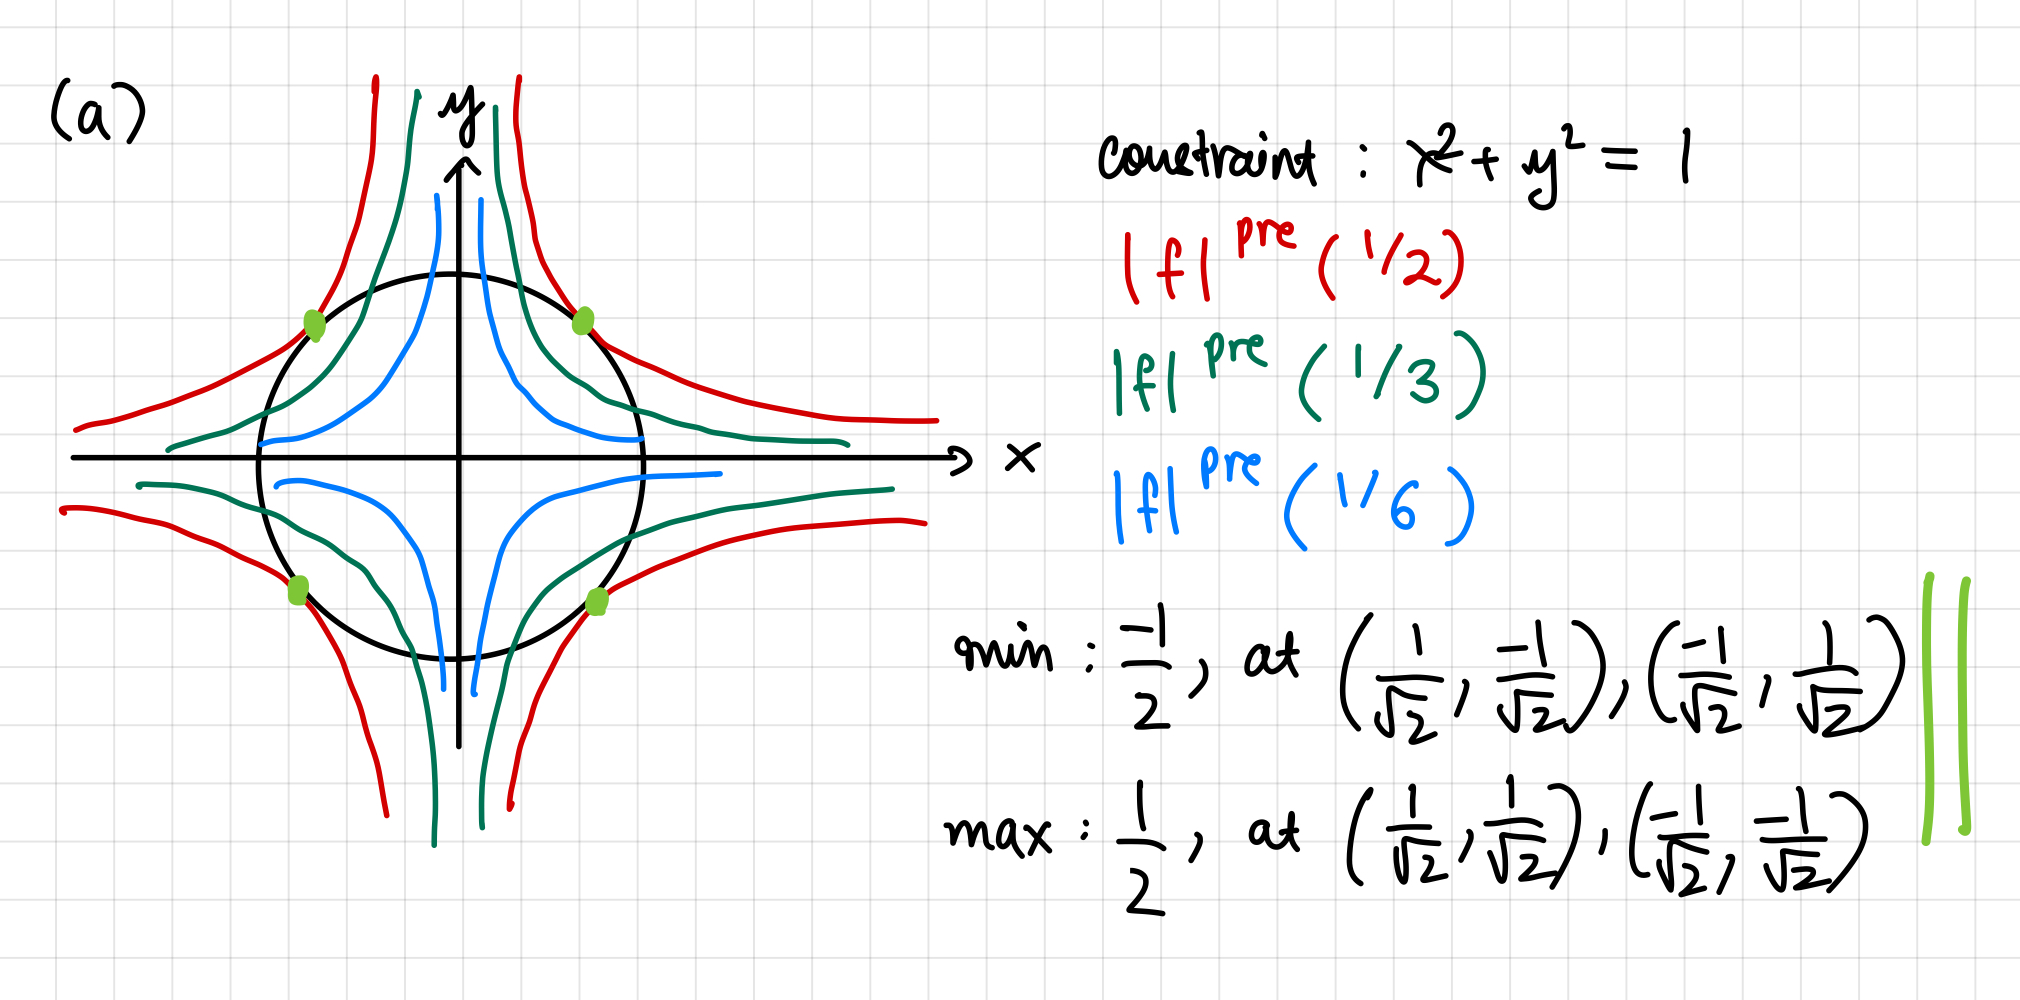
\includegraphics[width=16cm]{./figures/7.5a.jpeg}
    \end{center}
    \textbf{(b)}
    \begin{center}
        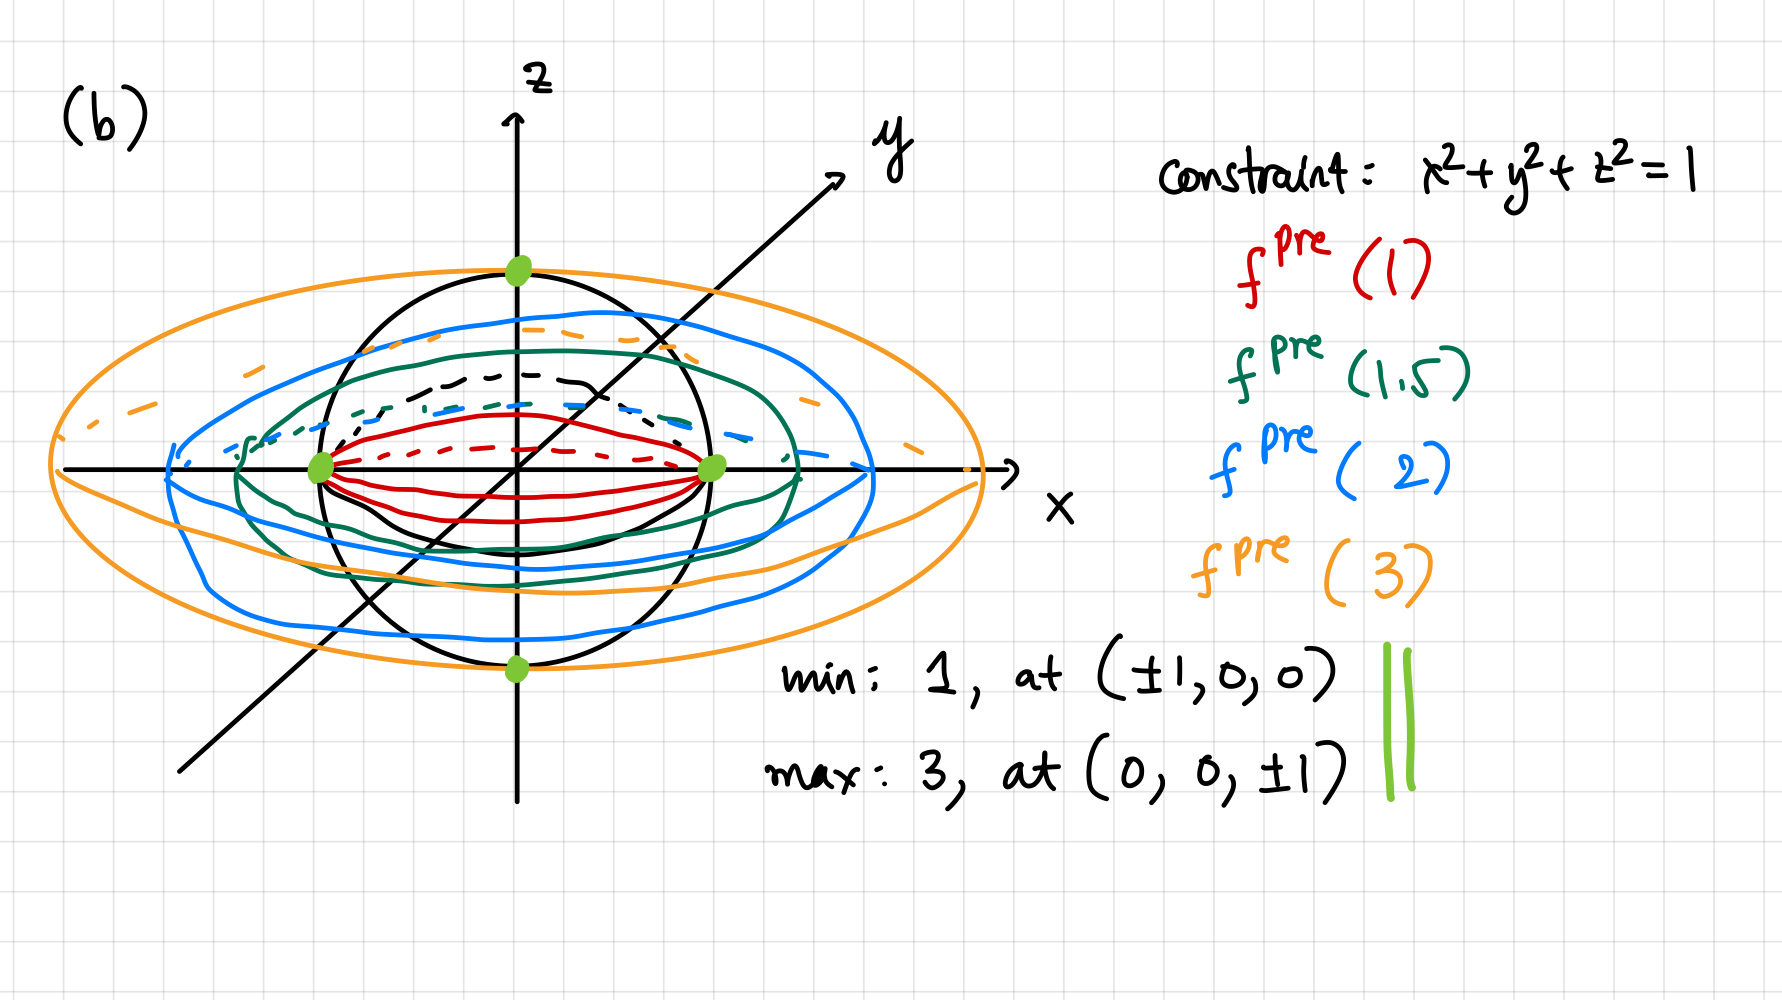
\includegraphics[width=16cm]{./figures/7.5b.jpeg}
    \end{center}
    \textbf{(c)} Optimizing $f(x, y, z) = (x-1)^2 + (y-2)^2 + (z-2)^2$
    \begin{center}
        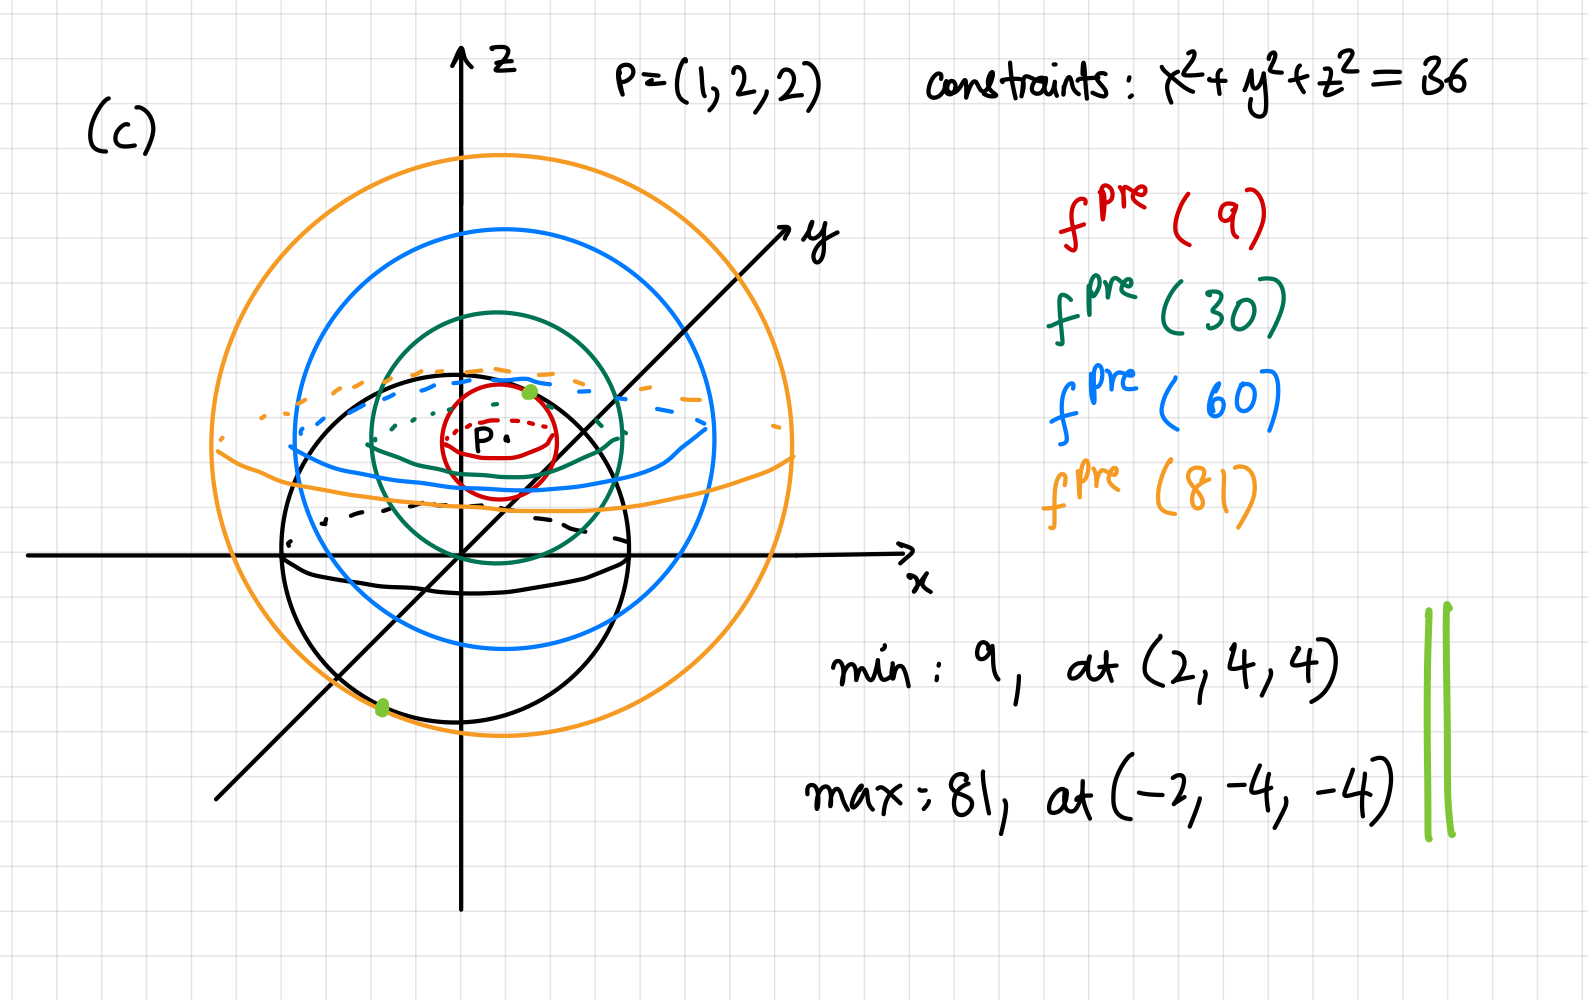
\includegraphics[width=16cm]{./figures/7.5c.jpeg}
    \end{center}
\end{solution}

\begin{problem} [VI \redtext{done}]
Fix $n$, and let \[\Delta = \{(p_1,\ldots, p_n) : p_i\geq 0, \hbox{ for } i=1,\ldots n,\,\hbox{ and } \sum_{i=1}^n p_i = 1 \}\] be the space of probability vectors in $\bbr^n$. Define the {\em entropy function} $H\colon \Delta \to \bbr_{\geq 0}$ by the formula
\[H(p) = \sum_{i=1}^n \phi(p_i),
\]
where $\phi(x) = -x\log x$, for $x\in (0,1)$, and $0$, for $x\in\{0,1\}$.
\begin{enumerate}
    \item[(a)] Using Lagrange multipliers, find the maximum value of $H$ on $\Delta$.
    \item[(b)] Using convexity of the   negative logarithm function, find the maximum value of $H$ on $\Delta$.
\end{enumerate}
\end{problem}
\begin{solution}
    First, $f(x) = -x \log x$ is concave on $(0, \infty)$. Indeed, \[
        f''(x) = -1/x < 0
    \]
    Therefore, all other held equal, for $i \neq j; a, b > 0$, we have
    \begin{align*}
        H\left(p_i = p_j = \frac{a+b}{2}\right) & - H(p_i = a, p_j = b)                                                                                 \\
                                                & = -\frac{a+b}{2}  \left(\log\left(\frac{a+b}{2}\right)\right) - \left(a (-\log a) + b(-\log b)\right) \\
                                                & \geq 0
    \end{align*}
    since $(-x \log x)$ is strictly concave.

    When $a$ or $b$ is zero, or both, the above inequality still holds trivially. Therefore \[
        H(p_i = a, p_j = b) \leq H\left(p_i = p_j = \frac{a+b}{2}\right)
    \]
    with equality holding only when $a = b$.

    \textbf{(a)} \textbf{1.} We first want to show that we can apply the method of Lagrange multipliers.

    \textbf{1.1.} WTS $H$ and $G \coloneqq \sum_{i=1}^{n} p_i$ are $C^1$ on some region $U \subseteq \Delta$.

    Define $A = \{p : \exists p_i = 0\}$

    Restrict $U = int(\Delta) = \Delta \backslash A$. It is first needed to prove that by restricting $U$ as so, we are not losing the maximal point, i.e., $\max_{A} H < \max_{U} H$.

    Fix $p$ such that it has a non-empty index set of 0-valued entries, i.e. $I = \{ 1 \leq i \leq n : p_i = 0 \} \neq \emptyset$. $I$ can't be entire set of 1 to $n$, since $\sum p_i = 1$. Therefore there exists $j$ such that $p_j = c > 0$. Then, for each $i \in I$, we have: \[
        H(p_i = 0, p_j = c) < H(p_i = p_j = c/2)
    \]
    Iterate same routine for the finitely many members of $I$, and we get that \[
        H(p) < H(p_{new})
    \]
    where $p_{new}$ has no 0-valued entry and $p_j = c/2^{|I|}$, after carrying out the procedure $|I|$ times. And $p_{new} \in U \implies \max_{A} H < \max_{U} H$.

    Then, on $U$, $H$ is $C^1$ since $(-x \log x)$ is twice differentiable on $(0, \infty)$.

    It is clear that $G$ is $C^1$ since it is linear.

    \textbf{1.2.} On $U,$

    \[
        grad_{q}G = \begin{pmatrix}
            1 \\
            1 \\
            \vdots
        \end{pmatrix} \neq 0 \forall q \in S.
        \]

    We do not have to assert that the domain is compact, since this only guarantees that the extremal values will be achieved within the domain. We will instead do this by directly verifying that the critical points are indeed within $U$.

    \textbf{2.} Let \[
        L(p) = H(p) - \lambda \left(\sum_{i=1}^{n} p_i - 1\right)
    \]
    then using Lagrange multipliers, extremal values are achieved when
    \begin{align*}
        0            & = \frac{\partial L}{\partial p_i}          \\
                     & = - (\log p_i + \frac{p_i}{p_i}) - \lambda \\
                     & = - \log p_i - 1 - \lambda                 \\
        \implies p_i & = e^{-\lambda -1}
    \end{align*}
    Thus we have that $p_i$ are all equal, $p_i = 1/n$.

    Directly verify that indeed, $(1/n, 1/n, \cdots) \in U$.

    Therefore maximum value of $H$ on $U$, consequently on $\Delta$ is \[
        H(1/n, 1/n, \cdots) = -n (1/n) \log(1/n) = \log n
    \]

    % \textbf{(b)} We want to prove that the maximum value of $H$ is achieved when $p_i$ are all equal, i.e., $p_i = 1/n \forall 1 \leq i \leq n$.

    % Therefore, given any $(p_1, p_2, \ldots, p_n)$, WLOG, sorted in increasing order, we have
    % \begin{align*}
    % H(1/n, 1/n, \ldots) &\geq H(p_1, \frac{2}{n} - p_1, 1/n, \ldots, 1/n)\\
    % & \geq H(p_1, p_2, \frac{3}{n} - p_1 - p_2, 1/n, \ldots, 1/n)\\
    % & \geq \ldots \\
    % &\geq H(p_1, p_2, \ldots, p_{n-1}, 1 - (p_1 + p_2 + \ldots + p_{n-1})) \\
    % &= H(p_1, p_2, \ldots, p_{n-1}, p_n)
    % \end{align*}

    \textbf{(b)} Since $-x \log x$ is concave, we can apply Jensen's inequality:
    \begin{align*}
        \frac{1}{n} \sum_{i=1}^{n} -p_i \log (p_i) & \leq -\frac{1}{n} \log\left(\frac{\sum p_i}{n}\right) \\
        \implies H(p)                              & \leq - \log(1/n) = \log n
    \end{align*}
    Equality holds when $p_1 = p_2 = \cdots = p_n$, which is achievable, $p_i = 1/n \forall i$. $H$ is therefore maximal at $(1/n, 1/n, \ldots, 1/n)$, with value $\log n$.
\end{solution}

\begin{problem} [VII \redtext{done}]
The {\em triple product} $\alpha\colon \bbr^3\times\bbr^3\times\bbr^3\to \bbr$ is defined by the formula
\[\alpha(u,v,w) := \det( u \, v \, w),
\]
where $(u\,  v\,  w)$ is the matrix whose columns are $u, v$ and $w$.   This exercise  will make multiple use of the properties of determinants;
\begin{itemize}
    \item the determinant is multilinear in the columns of $A$
    \item swapping two columns changes the sign of the determinant;
    \item the absolute value of $\det(A)$  is the volume of the (possibly degenerate) parallelepiped spanned by the columns of $A$  (which is the volume of the image of the unit cube under $A$);
    \item the sign of $\det(A)$  is the orientation of the columns relative to the standard basis $e_1, \ldots, e_n$ (which for $n=3$ is given by the ``right hand rule" -- google it!)
\end{itemize}
\begin{enumerate}
    \item[(a)]  Show that for all $v,w\in \bbr^3$, there exists a unique vector $z\in\bbr^3$ such that
        \[\alpha(u,v,w) = \langle u, z \rangle,
        \]
        for all $u\in \bbr^3$.  Define the {\em cross product of $v$ and $w$} to be this vector $v\times w:= z$.
    \item[(b)] Derive the following formula for $v\times w$:
        \[v\times w = \det \begin{pmatrix} {\bf i} & v_1 & w_1 \\
                {\bf j} & v_2 & w_2 \\
                {\bf k} & v_3 & w_3 \\
            \end{pmatrix},
        \]
        where the $v_i$'s and $w_i$'s are the components of $v$ and $w$, respectively, and ${\bf i}, {\bf j}, {\bf k}$ are symbolic placeholders for the coordinate vectors $e_1, e_2,e_3$.
        Compute the cross product of the vectors $(6,1,0), (0,2,2)$.
    \item[(c)] [Warmup -- don't turn in] Verify the following properties of the cross product:
        \begin{itemize}
            \item $v\times w$ is bilinear in $v,w$;
            \item $v\times w = -w\times v$ ({\em antisymmetry} of the cross-product);
            \item $e_1\times e_2 = e_3$, $e_2\times e_3 = e_1$, and $e_3\times e_1 = e_2$;
            \item $u\times (v\times w) + v\times(w\times u) +  w\times(u\times v) = 0$ (this is known as a {\em Jacobi identity}, and together with bilinearity and antisymmetry, shows that $\times$ is an example of a {\em Lie bracket});
            \item $\langle v,v\times w\rangle =  \langle w,v\times w\rangle =  0$, and hence $v\times w$ is orthogonal to both $v$ and $w$;
            \item $|\langle u, v\times w\rangle|$ is the volume of the (possibly degenerate) parallelepiped spanned by $u,v,w$;
            \item $|v\times w|$ is the area of the parallelogram spanned by $v$ and $w$ in $\bbr^3$, and hence:
                  \[|v\times w| = |v|\,|w|\sin(\theta),
                  \]
                  where $\theta\in (-\pi/2,\pi/2)$ is the angle between $v$ and $w$;
            \item the orientation of $v\times w$ relative to $v$ and $w$ is determined by the ``right hand rule."
        \end{itemize}
    \item[(d)] Prove the product formula for cross product: If $f,g\colon \bbr^n\to \bbr^3$ are differentiable at $p$, then for every $v\in\bbr^n$, we have
        \[D(f\times g)_p(v) = f(p)\times Dg_p(v) + Df_p(v)\times g(p).
        \]
        In particular, when $n=1$, we have
        \[(f\times g)'(t) = f(t)\times g'(t) + f'(t) \times g(t).
        \]
        (Please make use of the general properties of derivative here).
    \item[(e)] [Warmup -- don't turn in] Show that if $v,w$ span a plane $P$ (through the origin) in $\bbr^3$, then
        \[P = \{x\in \bbr^3: \alpha(x,v,w) = \langle x, v\times w\rangle = 0\}.
        \]
        Use this to find the equation $ax_1 + bx_2 + cx_3  = d$ of the plane through the point $(2,1,2)$ and spanned by the vectors  $(6,1,0), (0,2,2)$.
    \item[(f)] Find the equation of the tangent plane to the {\em parametrized surface} $\sigma\colon \bbr^2\to \bbr^3$ given by
        \[\sigma(r, s) = (2r^3, rs^2, 2s),
        \]
        through the point $\sigma(1,1) = (2,1,2)$. Consult your MV Calc buddy if this seems completely foreign to you. We will be discussing parametrized surfaces very soon!
    \item[(g)] Now using the gradient, find the equation of the tangent plane to the {\em implicitly-defined} surface $x^2 - xyz + z^2 = 1$ through the point $(1,1,1)$.
\end{enumerate}
\end{problem}
\begin{solution}
    \textbf{(a)} We first prove existence, then uniqueness.

    \textbf{1.} Let $z = e_1 \alpha(e_1, v, w) + e_2 \alpha(e_2, v, w) + e_3 \alpha(e_3, v, w)$. Then \begin{align*}
        \iprod{u}{z} & = u_1 \alpha(e_1, v, w) + u_2 \alpha(e_2, v, w) + u_3 \alpha(e_3, v, w) \\
                     & = \alpha(u, v, w)
    \end{align*}
    as required.

    \textbf{2.} Suppose there exists $z_1, z_2$ that satisfy the conditions for all $u$. Then \begin{align*}
        \iprod{u}{z_1}                & = \iprod{u}{z_2} \\
        \implies \iprod{u}{z_1 - z_2} & = 0 \forall u
    \end{align*}
    which implies $z_1 - z_2 = 0 \implies z_1 = z_2$. \qed

    \textbf{(b)} We have \begin{align*}
        \det \begin{pmatrix} {\bf i} & v_1 & w_1 \\
                {\bf j} & v_2 & w_2 \\
                {\bf k} & v_3 & w_3 \\
             \end{pmatrix} & = {\bf i}(w_3v_2 - v_3w_2) + {\bf j}(w_1v_3 - v_1w_3) + {\bf k}(w_2v_1 - v_2w_1)                \\
                                                    & = e_1\alpha(e_1, v, w) + e_2 \alpha(e_2, v, w) + e_3 \alpha(e_3, v, w) \\
                                                    & = z = v \times w
    \end{align*}
    as required.

    Then \begin{align*}
        (6, 1, 0) \times (0, 2, 2) & = \det
        \begin{pmatrix}
            {\bf i} & 6 & 0 \\
            {\bf j} & 1 & 2 \\
            {\bf k} & 0 & 2
        \end{pmatrix}                                                                         \\
                                   & = 2 {\bf i} - 12 {\bf j} + 12 {\bf k} = (2, -12, 12). \qed
    \end{align*}

    \textbf{(d)} Since the cross product is bilinear, let $\beta: \bbr^3 \times \bbr^3 \to \bbr^3; (x, y) \mapsto x \times y$, $\beta$ is bilinearg. Then
    \begin{align*}
        D(\beta(f, g))_p(v) & = \beta(Df_{p}(v), g(p)) + \beta(f(p) , Dg_p(v)) \\
                            & = Df_p(v) \times g(p) + f(p) \times Dg_p(v)
    \end{align*}
    as required, with the case when $n = 1$ following naturally. \qed

    \textbf{(f)} The tangent plane is the best linear approximation of the surface at that point. Therefore, we can calculate \begin{align*}
        J\sigma_{(r, s)}          & = \begin{pmatrix}
                                          6r^2 & 0   \\
                                          s^2  & 2rs \\
                                          0    & 2
                                      \end{pmatrix} \\
        \implies J\sigma_{(1, 1)} & = \begin{pmatrix}
                                          6 & 0 \\
                                          1 & 2 \\
                                          0 & 2
                                      \end{pmatrix}
    \end{align*}
    so as to get basis vectors for the plane: $v = J\sigma_{(1, 1)}e_1 = (6, 1, 0)$ and $w = J\sigma_{(1, 1)}e_2 = (0, 2, 2)$ in the coordinate system that has $p = (2, 1, 2)$ as its origin. From \textbf{(e)}, any $x'$ on this plane has to satisfy:
    \begin{align*}
        \iprod{x'}{v \times w}          & = 0 \\
        \iprod{x'}{(2, -12, 12)}        & = 0 \\
        \implies 2x'_1 -12x'_2 + 12x'_3 & = 0
    \end{align*}

    Reverting back to the original coordinate system:
    \begin{align*}
        2(x_1 - 2) - 12(x_2 - 1) + 12 (x_3 - 2) & = 0  \\
        \implies 2x_1 - 12x_2 + 12x_3           & = 16
    \end{align*}

    \textbf{(g)}
    \[
        x^2 - xyz + z^2 = 1
    \]
    Define $f: \bbr^3 \to \bbr$, \[
        f(x, y, z) = x^2 - xyz + z^2 - 1
    \]
    Then \begin{align*}
        grad_{(1, 1, 1)}(f) & = \begin{pmatrix}
                                    2x - yz \\
                                    -xz     \\
                                    -xy + 2z
                                \end{pmatrix}\bigg|_{(x, y, z) = (1, 1, 1)} = \begin{pmatrix}
                                                                                  1  \\
                                                                                  -1 \\
                                                                                  1
                                                                              \end{pmatrix}
    \end{align*}
    From previous homework, we know that $grad_p(f)$ is perpendicular to the level set of $f$, which in this case is the surface itself. It follows that (1, -1, 1) is the normal vector of the tangent plane. It follows that \begin{align*}
        \iprod{(x, y, z) - (1, 1, 1)}{(1, -1, 1)} & = 0 \\
        (x-1) - (y-1) + (z-1)                     & = 0 \\
        x-y+z = 1
    \end{align*}
\end{solution}
\end{document}